\documentclass[twoside]{book}

% Packages required by doxygen
\usepackage{fixltx2e}
\usepackage{calc}
\usepackage{doxygen}
\usepackage[export]{adjustbox} % also loads graphicx
\usepackage{graphicx}
\usepackage[utf8]{inputenc}
\usepackage{makeidx}
\usepackage{multicol}
\usepackage{multirow}
\PassOptionsToPackage{warn}{textcomp}
\usepackage{textcomp}
\usepackage[nointegrals]{wasysym}
\usepackage[table]{xcolor}

% NLS support packages
\usepackage[brazil]{babel}
% Font selection
\usepackage[T1]{fontenc}
\usepackage[scaled=.90]{helvet}
\usepackage{courier}
\usepackage{amssymb}
\usepackage{sectsty}
\renewcommand{\familydefault}{\sfdefault}
\allsectionsfont{%
  \fontseries{bc}\selectfont%
  \color{darkgray}%
}
\renewcommand{\DoxyLabelFont}{%
  \fontseries{bc}\selectfont%
  \color{darkgray}%
}
\newcommand{\+}{\discretionary{\mbox{\scriptsize$\hookleftarrow$}}{}{}}

% Page & text layout
\usepackage{geometry}
\geometry{%
  a4paper,%
  top=2.5cm,%
  bottom=2.5cm,%
  left=2.5cm,%
  right=2.5cm%
}
\tolerance=750
\hfuzz=15pt
\hbadness=750
\setlength{\emergencystretch}{15pt}
\setlength{\parindent}{0cm}
\setlength{\parskip}{3ex plus 2ex minus 2ex}
\makeatletter
\renewcommand{\paragraph}{%
  \@startsection{paragraph}{4}{0ex}{-1.0ex}{1.0ex}{%
    \normalfont\normalsize\bfseries\SS@parafont%
  }%
}
\renewcommand{\subparagraph}{%
  \@startsection{subparagraph}{5}{0ex}{-1.0ex}{1.0ex}{%
    \normalfont\normalsize\bfseries\SS@subparafont%
  }%
}
\makeatother

% Headers & footers
\usepackage{fancyhdr}
\pagestyle{fancyplain}
\fancyhead[LE]{\fancyplain{}{\bfseries\thepage}}
\fancyhead[CE]{\fancyplain{}{}}
\fancyhead[RE]{\fancyplain{}{\bfseries\leftmark}}
\fancyhead[LO]{\fancyplain{}{\bfseries\rightmark}}
\fancyhead[CO]{\fancyplain{}{}}
\fancyhead[RO]{\fancyplain{}{\bfseries\thepage}}
\fancyfoot[LE]{\fancyplain{}{}}
\fancyfoot[CE]{\fancyplain{}{}}
\fancyfoot[RE]{\fancyplain{}{\bfseries\scriptsize Gerado por Doxygen }}
\fancyfoot[LO]{\fancyplain{}{\bfseries\scriptsize Gerado por Doxygen }}
\fancyfoot[CO]{\fancyplain{}{}}
\fancyfoot[RO]{\fancyplain{}{}}
\renewcommand{\footrulewidth}{0.4pt}
\renewcommand{\chaptermark}[1]{%
  \markboth{#1}{}%
}
\renewcommand{\sectionmark}[1]{%
  \markright{\thesection\ #1}%
}

% Indices & bibliography
\usepackage{natbib}
\usepackage[titles]{tocloft}
\setcounter{tocdepth}{3}
\setcounter{secnumdepth}{5}
\makeindex

% Hyperlinks (required, but should be loaded last)
\usepackage{ifpdf}
\ifpdf
  \usepackage[pdftex,pagebackref=true]{hyperref}
\else
  \usepackage[ps2pdf,pagebackref=true]{hyperref}
\fi
\hypersetup{%
  colorlinks=true,%
  linkcolor=blue,%
  citecolor=blue,%
  unicode%
}

% Custom commands
\newcommand{\clearemptydoublepage}{%
  \newpage{\pagestyle{empty}\cleardoublepage}%
}

\usepackage{caption}
\captionsetup{labelsep=space,justification=centering,font={bf},singlelinecheck=off,skip=4pt,position=top}

%===== C O N T E N T S =====

\begin{document}

% Titlepage & ToC
\hypersetup{pageanchor=false,
             bookmarksnumbered=true,
             pdfencoding=unicode
            }
\pagenumbering{alph}
\begin{titlepage}
\vspace*{7cm}
\begin{center}%
{\Large T\+AD lista }\\
\vspace*{1cm}
{\large Gerado por Doxygen 1.8.13}\\
\end{center}
\end{titlepage}
\clearemptydoublepage
\pagenumbering{roman}
\tableofcontents
\clearemptydoublepage
\pagenumbering{arabic}
\hypersetup{pageanchor=true}

%--- Begin generated contents ---
\chapter{Índice Hierárquico}
\section{Class Hierarchy}
This inheritance list is sorted roughly, but not completely, alphabetically\+:\begin{DoxyCompactList}
\item \contentsline{section}{ls\+:\+:list$<$ T $>$}{\pageref{classls_1_1list}}{}
\item \contentsline{section}{ls\+:\+:my\+\_\+const\+\_\+iterator$<$ T $>$}{\pageref{classls_1_1my__const__iterator}}{}
\begin{DoxyCompactList}
\item \contentsline{section}{ls\+:\+:my\+\_\+iterator$<$ T $>$}{\pageref{classls_1_1my__iterator}}{}
\end{DoxyCompactList}
\item \contentsline{section}{ls\+:\+:Node$<$ T $>$}{\pageref{structls_1_1Node}}{}
\end{DoxyCompactList}

\chapter{Índice dos Componentes}
\section{Class List}
Here are the classes, structs, unions and interfaces with brief descriptions\+:\begin{DoxyCompactList}
\item\contentsline{section}{\hyperlink{classls_1_1list}{ls\+::list$<$ T $>$} \\*List implementation }{\pageref{classls_1_1list}}{}
\item\contentsline{section}{\hyperlink{classls_1_1my__const__iterator}{ls\+::my\+\_\+const\+\_\+iterator$<$ T $>$} \\*Constant iterator implementation }{\pageref{classls_1_1my__const__iterator}}{}
\item\contentsline{section}{\hyperlink{classls_1_1my__iterator}{ls\+::my\+\_\+iterator$<$ T $>$} \\*Implements the infrastructure to support the bidirectional pointer }{\pageref{classls_1_1my__iterator}}{}
\item\contentsline{section}{\hyperlink{structls_1_1Node}{ls\+::\+Node$<$ T $>$} \\*Structure to each element in the list }{\pageref{structls_1_1Node}}{}
\end{DoxyCompactList}

\chapter{Classes}
\hypertarget{classls_1_1list}{}\section{Referência da Template de Classe ls\+:\+:list$<$ T $>$}
\label{classls_1_1list}\index{ls\+::list$<$ T $>$@{ls\+::list$<$ T $>$}}


List implementation.  




{\ttfamily \#include $<$list.\+h$>$}

\subsection*{Tipos Públicos}
\begin{DoxyCompactItemize}
\item 
\mbox{\Hypertarget{classls_1_1list_a71c7a4d7061c0c3f23aba13232eda0f6}\label{classls_1_1list_a71c7a4d7061c0c3f23aba13232eda0f6}} 
using \hyperlink{classls_1_1list_a71c7a4d7061c0c3f23aba13232eda0f6}{value\+\_\+type} = T
\begin{DoxyCompactList}\small\item\em Alias to type stored in container. \end{DoxyCompactList}\item 
\mbox{\Hypertarget{classls_1_1list_a91bb77719712ad6127f0bdf97ed5bd64}\label{classls_1_1list_a91bb77719712ad6127f0bdf97ed5bd64}} 
using \hyperlink{classls_1_1list_a91bb77719712ad6127f0bdf97ed5bd64}{size\+\_\+type} = size\+\_\+t
\begin{DoxyCompactList}\small\item\em Alias to size type. \end{DoxyCompactList}\item 
\mbox{\Hypertarget{classls_1_1list_af036cf72da26107a5084c1e4b45b9cb7}\label{classls_1_1list_af036cf72da26107a5084c1e4b45b9cb7}} 
using \hyperlink{classls_1_1list_af036cf72da26107a5084c1e4b45b9cb7}{iterator} = \hyperlink{classls_1_1my__iterator}{my\+\_\+iterator}$<$ \hyperlink{classls_1_1list_a71c7a4d7061c0c3f23aba13232eda0f6}{value\+\_\+type} $>$
\begin{DoxyCompactList}\small\item\em Alias to bidirectional iterator used. \end{DoxyCompactList}\item 
\mbox{\Hypertarget{classls_1_1list_ad543276e86075caadf97ae64f2fc7cfc}\label{classls_1_1list_ad543276e86075caadf97ae64f2fc7cfc}} 
using \hyperlink{classls_1_1list_ad543276e86075caadf97ae64f2fc7cfc}{const\+\_\+iterator} = \hyperlink{classls_1_1my__const__iterator}{my\+\_\+const\+\_\+iterator}$<$ \hyperlink{classls_1_1list_a71c7a4d7061c0c3f23aba13232eda0f6}{value\+\_\+type} $>$
\begin{DoxyCompactList}\small\item\em Alias to const type of bidirectional iterator used. \end{DoxyCompactList}\item 
\mbox{\Hypertarget{classls_1_1list_afb0f652e0362bc8c3e82c16efe795bf3}\label{classls_1_1list_afb0f652e0362bc8c3e82c16efe795bf3}} 
using \hyperlink{classls_1_1list_afb0f652e0362bc8c3e82c16efe795bf3}{reference} = T \&
\begin{DoxyCompactList}\small\item\em Alias to data reference. \end{DoxyCompactList}\end{DoxyCompactItemize}
\subsection*{Métodos Públicos}
\begin{DoxyCompactItemize}
\item 
\mbox{\Hypertarget{classls_1_1list_a3717713cf5e4558e543b533d14eef424}\label{classls_1_1list_a3717713cf5e4558e543b533d14eef424}} 
\hyperlink{classls_1_1list_a3717713cf5e4558e543b533d14eef424}{list} ()
\begin{DoxyCompactList}\small\item\em Default constructor that creates an empty list. \end{DoxyCompactList}\item 
\mbox{\Hypertarget{classls_1_1list_a4badb105feef42346fbc3a26be770387}\label{classls_1_1list_a4badb105feef42346fbc3a26be770387}} 
\hyperlink{classls_1_1list_a4badb105feef42346fbc3a26be770387}{list} (\hyperlink{classls_1_1list_a91bb77719712ad6127f0bdf97ed5bd64}{size\+\_\+type} count)
\begin{DoxyCompactList}\small\item\em Constructs the list with count default-\/inserted instances of T. \end{DoxyCompactList}\item 
\mbox{\Hypertarget{classls_1_1list_a783b17259b4ac0805c58d6a959d3c11f}\label{classls_1_1list_a783b17259b4ac0805c58d6a959d3c11f}} 
{\footnotesize template$<$typename Input\+It $>$ }\\\hyperlink{classls_1_1list_a783b17259b4ac0805c58d6a959d3c11f}{list} (Input\+It first, Input\+It last)
\begin{DoxyCompactList}\small\item\em Constructs the list with the contents of the range \mbox{[}first, last). \end{DoxyCompactList}\item 
\mbox{\Hypertarget{classls_1_1list_a167e96cf439f62fbefca1d06a958c798}\label{classls_1_1list_a167e96cf439f62fbefca1d06a958c798}} 
\hyperlink{classls_1_1list_a167e96cf439f62fbefca1d06a958c798}{list} (const \hyperlink{classls_1_1list}{list} \&other)
\begin{DoxyCompactList}\small\item\em Copy constructor. Constructs the list with the deep copy of the contents of other. \end{DoxyCompactList}\item 
\mbox{\Hypertarget{classls_1_1list_ac4d5e3102e51f80bcc82fdab0b8d187f}\label{classls_1_1list_ac4d5e3102e51f80bcc82fdab0b8d187f}} 
\hyperlink{classls_1_1list_ac4d5e3102e51f80bcc82fdab0b8d187f}{list} (std\+::initializer\+\_\+list$<$ T $>$ ilist)
\begin{DoxyCompactList}\small\item\em Constructs the list with the contents of the initializer list init. \end{DoxyCompactList}\item 
\mbox{\Hypertarget{classls_1_1list_ab341963c62740c4e4d1a042fdba9c856}\label{classls_1_1list_ab341963c62740c4e4d1a042fdba9c856}} 
\hyperlink{classls_1_1list_ab341963c62740c4e4d1a042fdba9c856}{$\sim$list} ()
\begin{DoxyCompactList}\small\item\em Destructs the list. The destructors of the elements are called and the used storage is deallocated. \end{DoxyCompactList}\item 
\mbox{\Hypertarget{classls_1_1list_aa447eb049c1c13b2846aba8689b875af}\label{classls_1_1list_aa447eb049c1c13b2846aba8689b875af}} 
\hyperlink{classls_1_1list}{list}$<$ T $>$ \& \hyperlink{classls_1_1list_aa447eb049c1c13b2846aba8689b875af}{operator=} (const \hyperlink{classls_1_1list}{list}$<$ T $>$ \&other)
\begin{DoxyCompactList}\small\item\em Copy assignment operator. Replaces the contents with a copy of the contents of other. \end{DoxyCompactList}\item 
\mbox{\Hypertarget{classls_1_1list_a87472ac420c9de170637cb35aefbde8c}\label{classls_1_1list_a87472ac420c9de170637cb35aefbde8c}} 
\hyperlink{classls_1_1list}{list}$<$ T $>$ \& \hyperlink{classls_1_1list_a87472ac420c9de170637cb35aefbde8c}{operator=} (std\+::initializer\+\_\+list$<$ T $>$ ilist)
\begin{DoxyCompactList}\small\item\em Replaces the contents with those identified by initializer list ilist. \end{DoxyCompactList}\item 
\mbox{\Hypertarget{classls_1_1list_a73458e8145cc3ee958fb59940084ab61}\label{classls_1_1list_a73458e8145cc3ee958fb59940084ab61}} 
\hyperlink{classls_1_1list_af036cf72da26107a5084c1e4b45b9cb7}{iterator} \hyperlink{classls_1_1list_a73458e8145cc3ee958fb59940084ab61}{begin} ()
\begin{DoxyCompactList}\small\item\em Returns an iterator pointing to the first item in the list. \end{DoxyCompactList}\item 
\mbox{\Hypertarget{classls_1_1list_a0c168cf2301ed80e1a853827d366294a}\label{classls_1_1list_a0c168cf2301ed80e1a853827d366294a}} 
\hyperlink{classls_1_1list_ad543276e86075caadf97ae64f2fc7cfc}{const\+\_\+iterator} \hyperlink{classls_1_1list_a0c168cf2301ed80e1a853827d366294a}{cbegin} () const
\begin{DoxyCompactList}\small\item\em Returns a constant iterator pointing to the first item in the list. \end{DoxyCompactList}\item 
\mbox{\Hypertarget{classls_1_1list_a23e842f652b4da5c445499dc81e67934}\label{classls_1_1list_a23e842f652b4da5c445499dc81e67934}} 
\hyperlink{classls_1_1list_af036cf72da26107a5084c1e4b45b9cb7}{iterator} \hyperlink{classls_1_1list_a23e842f652b4da5c445499dc81e67934}{end} ()
\begin{DoxyCompactList}\small\item\em Returns an iterator pointing to the end mark in the list, i.\+e. the position just after the last element of the list. \end{DoxyCompactList}\item 
\mbox{\Hypertarget{classls_1_1list_ac8d06153e963e892c146bc227cfbb96c}\label{classls_1_1list_ac8d06153e963e892c146bc227cfbb96c}} 
\hyperlink{classls_1_1list_ad543276e86075caadf97ae64f2fc7cfc}{const\+\_\+iterator} \hyperlink{classls_1_1list_ac8d06153e963e892c146bc227cfbb96c}{cend} () const
\begin{DoxyCompactList}\small\item\em Returns a constant iterator pointing to the end mark in the list, i.\+e. the position just after the last element of the list. \end{DoxyCompactList}\item 
\mbox{\Hypertarget{classls_1_1list_a3cfcda5a97910595ab9268150a1f6019}\label{classls_1_1list_a3cfcda5a97910595ab9268150a1f6019}} 
\hyperlink{classls_1_1list_a91bb77719712ad6127f0bdf97ed5bd64}{size\+\_\+type} \hyperlink{classls_1_1list_a3cfcda5a97910595ab9268150a1f6019}{size} () const
\begin{DoxyCompactList}\small\item\em Return the number of elements in the container. \end{DoxyCompactList}\item 
\mbox{\Hypertarget{classls_1_1list_a661ae23af20249a5acd872b5981d222d}\label{classls_1_1list_a661ae23af20249a5acd872b5981d222d}} 
bool \hyperlink{classls_1_1list_a661ae23af20249a5acd872b5981d222d}{empty} ()
\begin{DoxyCompactList}\small\item\em Returns true if the container contains no elements, and false otherwise. \end{DoxyCompactList}\item 
\mbox{\Hypertarget{classls_1_1list_a94d588131af6f58af50f85debcc1cd0d}\label{classls_1_1list_a94d588131af6f58af50f85debcc1cd0d}} 
void \hyperlink{classls_1_1list_a94d588131af6f58af50f85debcc1cd0d}{clear} ()
\begin{DoxyCompactList}\small\item\em Remove (either logically or physically) all elements from the container. \end{DoxyCompactList}\item 
\mbox{\Hypertarget{classls_1_1list_ad4db2fb23d8774b280f6e8d0f49166c0}\label{classls_1_1list_ad4db2fb23d8774b280f6e8d0f49166c0}} 
const T \& \hyperlink{classls_1_1list_ad4db2fb23d8774b280f6e8d0f49166c0}{front} () const
\begin{DoxyCompactList}\small\item\em Returns the object at the beginning of the list. \end{DoxyCompactList}\item 
\mbox{\Hypertarget{classls_1_1list_a7429ad77511be5fe6f165a80c1dc7d02}\label{classls_1_1list_a7429ad77511be5fe6f165a80c1dc7d02}} 
T \& \hyperlink{classls_1_1list_a7429ad77511be5fe6f165a80c1dc7d02}{front} ()
\begin{DoxyCompactList}\small\item\em Returns the object at the beginning of the list. \end{DoxyCompactList}\item 
\mbox{\Hypertarget{classls_1_1list_a1439d9f2b9441ffe3e6c0c8111b29cb1}\label{classls_1_1list_a1439d9f2b9441ffe3e6c0c8111b29cb1}} 
T \& \hyperlink{classls_1_1list_a1439d9f2b9441ffe3e6c0c8111b29cb1}{back} ()
\begin{DoxyCompactList}\small\item\em Returns the object at the end of the list. \end{DoxyCompactList}\item 
\mbox{\Hypertarget{classls_1_1list_a76c0d5952f1843c0f1183f5acb144103}\label{classls_1_1list_a76c0d5952f1843c0f1183f5acb144103}} 
const T \& \hyperlink{classls_1_1list_a76c0d5952f1843c0f1183f5acb144103}{back} () const
\begin{DoxyCompactList}\small\item\em Returns the object at the end of the list. \end{DoxyCompactList}\item 
\mbox{\Hypertarget{classls_1_1list_a3ae27bac754d4ca95da34c9040f33d48}\label{classls_1_1list_a3ae27bac754d4ca95da34c9040f33d48}} 
void \hyperlink{classls_1_1list_a3ae27bac754d4ca95da34c9040f33d48}{push\+\_\+front} (const T \&value)
\begin{DoxyCompactList}\small\item\em Adds value to the front of the list. \end{DoxyCompactList}\item 
\mbox{\Hypertarget{classls_1_1list_a21438e1be5b2143896ee8480cb2beb18}\label{classls_1_1list_a21438e1be5b2143896ee8480cb2beb18}} 
void \hyperlink{classls_1_1list_a21438e1be5b2143896ee8480cb2beb18}{push\+\_\+back} (const T \&value)
\begin{DoxyCompactList}\small\item\em Adds value to the end of the list. \end{DoxyCompactList}\item 
\mbox{\Hypertarget{classls_1_1list_aed8db7c16a16cd2d3290576725f7ffdd}\label{classls_1_1list_aed8db7c16a16cd2d3290576725f7ffdd}} 
void \hyperlink{classls_1_1list_aed8db7c16a16cd2d3290576725f7ffdd}{pop\+\_\+front} ()
\begin{DoxyCompactList}\small\item\em Removes the object at the front of the list. \end{DoxyCompactList}\item 
\mbox{\Hypertarget{classls_1_1list_a59d8ce6f60dca1e3a30b3e3d9f4154c2}\label{classls_1_1list_a59d8ce6f60dca1e3a30b3e3d9f4154c2}} 
void \hyperlink{classls_1_1list_a59d8ce6f60dca1e3a30b3e3d9f4154c2}{pop\+\_\+back} ()
\begin{DoxyCompactList}\small\item\em Removes the object at the end of the list. \end{DoxyCompactList}\item 
\mbox{\Hypertarget{classls_1_1list_aef14276ef9726f7ed30dbe9a76f4035f}\label{classls_1_1list_aef14276ef9726f7ed30dbe9a76f4035f}} 
void \hyperlink{classls_1_1list_aef14276ef9726f7ed30dbe9a76f4035f}{assign} (const T \&value)
\begin{DoxyCompactList}\small\item\em Replaces the content of the list with copies of value. \end{DoxyCompactList}\item 
\mbox{\Hypertarget{classls_1_1list_a8a9ebb0c52a3a472e69cae0f50de5737}\label{classls_1_1list_a8a9ebb0c52a3a472e69cae0f50de5737}} 
void \hyperlink{classls_1_1list_a8a9ebb0c52a3a472e69cae0f50de5737}{assign} (\hyperlink{classls_1_1list_a91bb77719712ad6127f0bdf97ed5bd64}{size\+\_\+type} count, const T \&value)
\begin{DoxyCompactList}\small\item\em Clear list and insert count copies of value. \end{DoxyCompactList}\item 
\mbox{\Hypertarget{classls_1_1list_a8528bc556cc62982161cd369e65ad3b7}\label{classls_1_1list_a8528bc556cc62982161cd369e65ad3b7}} 
{\footnotesize template$<$typename In\+Itr $>$ }\\void \hyperlink{classls_1_1list_a8528bc556cc62982161cd369e65ad3b7}{assign} (In\+Itr first, In\+Itr last)
\begin{DoxyCompactList}\small\item\em Replaces the contents with count copies of value value. \end{DoxyCompactList}\item 
\mbox{\Hypertarget{classls_1_1list_a3a502e5df12f088f6fda2edb5f79cfef}\label{classls_1_1list_a3a502e5df12f088f6fda2edb5f79cfef}} 
void \hyperlink{classls_1_1list_a3a502e5df12f088f6fda2edb5f79cfef}{assign} (std\+::initializer\+\_\+list$<$ T $>$ ilist)
\begin{DoxyCompactList}\small\item\em Replaces the contents of the list with the elements from the initializer list ilist. We may call, for instance, my\+List.\+assign( \{1, 2, 3, 4\} ), to replace the elements of the list with the elements 1, 2, 3, and 4, assuming that my\+List is a list of int. \end{DoxyCompactList}\item 
\mbox{\Hypertarget{classls_1_1list_afd87152a830dce5c7583239f9d25e044}\label{classls_1_1list_afd87152a830dce5c7583239f9d25e044}} 
\hyperlink{classls_1_1list_af036cf72da26107a5084c1e4b45b9cb7}{iterator} \hyperlink{classls_1_1list_afd87152a830dce5c7583239f9d25e044}{insert} (\hyperlink{classls_1_1list_af036cf72da26107a5084c1e4b45b9cb7}{iterator} pos, const T \&value)
\begin{DoxyCompactList}\small\item\em Adds value into the list before the position given by the iterator pos . The method returns an iterator to the position of the inserted item. \end{DoxyCompactList}\item 
\mbox{\Hypertarget{classls_1_1list_ac91d98c3a9b50bce8df0b6cda06e7e4f}\label{classls_1_1list_ac91d98c3a9b50bce8df0b6cda06e7e4f}} 
\hyperlink{classls_1_1list_af036cf72da26107a5084c1e4b45b9cb7}{iterator} \hyperlink{classls_1_1list_ac91d98c3a9b50bce8df0b6cda06e7e4f}{insert} (\hyperlink{classls_1_1list_ad543276e86075caadf97ae64f2fc7cfc}{const\+\_\+iterator} pos, const T \&value)
\begin{DoxyCompactList}\small\item\em Adds value into the list before the position given by the iterator pos . The method returns an iterator to the position of the inserted item. \end{DoxyCompactList}\item 
\mbox{\Hypertarget{classls_1_1list_a145b47adc8f9ab447baad3c3fa2ccd60}\label{classls_1_1list_a145b47adc8f9ab447baad3c3fa2ccd60}} 
{\footnotesize template$<$typename In\+Itr $>$ }\\\hyperlink{classls_1_1list_af036cf72da26107a5084c1e4b45b9cb7}{iterator} \hyperlink{classls_1_1list_a145b47adc8f9ab447baad3c3fa2ccd60}{insert} (\hyperlink{classls_1_1list_af036cf72da26107a5084c1e4b45b9cb7}{iterator} pos, In\+Itr first, In\+Itr last)
\begin{DoxyCompactList}\small\item\em Inserts elements from the range \mbox{[}first; last) before pos . \end{DoxyCompactList}\item 
\mbox{\Hypertarget{classls_1_1list_a22440e65537058d8758e416cbf7effc8}\label{classls_1_1list_a22440e65537058d8758e416cbf7effc8}} 
{\footnotesize template$<$typename In\+Itr $>$ }\\\hyperlink{classls_1_1list_af036cf72da26107a5084c1e4b45b9cb7}{iterator} \hyperlink{classls_1_1list_a22440e65537058d8758e416cbf7effc8}{insert} (\hyperlink{classls_1_1list_ad543276e86075caadf97ae64f2fc7cfc}{const\+\_\+iterator} pos, In\+Itr first, In\+Itr last)
\begin{DoxyCompactList}\small\item\em Inserts elements from the range \mbox{[}first; last) before pos . \end{DoxyCompactList}\item 
\mbox{\Hypertarget{classls_1_1list_a3781b36cb414bb517672808f98b22938}\label{classls_1_1list_a3781b36cb414bb517672808f98b22938}} 
\hyperlink{classls_1_1list_af036cf72da26107a5084c1e4b45b9cb7}{iterator} \hyperlink{classls_1_1list_a3781b36cb414bb517672808f98b22938}{insert} (\hyperlink{classls_1_1list_af036cf72da26107a5084c1e4b45b9cb7}{iterator} pos, std\+::initializer\+\_\+list$<$ T $>$)
\begin{DoxyCompactList}\small\item\em Inserts elements from the initializer list ilist before pos . Initializer list supports the user of insert as in my\+List.\+insert( pos, \{1, 2, 3, 4\} ) , which would insert the elements 1, 2, 3, and 4 in the list before pos , assuming that my\+List is a list of int. \end{DoxyCompactList}\item 
\mbox{\Hypertarget{classls_1_1list_a87c6c3007aaec374b29728ec8544b3c1}\label{classls_1_1list_a87c6c3007aaec374b29728ec8544b3c1}} 
\hyperlink{classls_1_1list_af036cf72da26107a5084c1e4b45b9cb7}{iterator} \hyperlink{classls_1_1list_a87c6c3007aaec374b29728ec8544b3c1}{insert} (\hyperlink{classls_1_1list_ad543276e86075caadf97ae64f2fc7cfc}{const\+\_\+iterator} pos, std\+::initializer\+\_\+list$<$ T $>$)
\begin{DoxyCompactList}\small\item\em Inserts elements from the initializer list ilist before pos . Initializer list supports the user of insert as in my\+List.\+insert( pos, \{1, 2, 3, 4\} ) , which would insert the elements 1, 2, 3, and 4 in the list before pos , assuming that my\+List is a list of int. \end{DoxyCompactList}\item 
\mbox{\Hypertarget{classls_1_1list_a76b6efa016395fd031baa05d63ebc745}\label{classls_1_1list_a76b6efa016395fd031baa05d63ebc745}} 
\hyperlink{classls_1_1list_af036cf72da26107a5084c1e4b45b9cb7}{iterator} \hyperlink{classls_1_1list_a76b6efa016395fd031baa05d63ebc745}{erase} (\hyperlink{classls_1_1list_af036cf72da26107a5084c1e4b45b9cb7}{iterator} pos)
\begin{DoxyCompactList}\small\item\em Removes the object at position pos . The method returns an iterator to the element that follows pos before the call. This operation invalidates pos , since the item it pointed to was removed from the list. \end{DoxyCompactList}\item 
\mbox{\Hypertarget{classls_1_1list_ae616e00db8cc2bd8641baf06cdbd99ab}\label{classls_1_1list_ae616e00db8cc2bd8641baf06cdbd99ab}} 
\hyperlink{classls_1_1list_af036cf72da26107a5084c1e4b45b9cb7}{iterator} \hyperlink{classls_1_1list_ae616e00db8cc2bd8641baf06cdbd99ab}{erase} (\hyperlink{classls_1_1list_ad543276e86075caadf97ae64f2fc7cfc}{const\+\_\+iterator} pos)
\begin{DoxyCompactList}\small\item\em Removes the object at position pos . The method returns an iterator to the element that follows pos before the call. This operation invalidates pos , since the item it pointed to was removed from the list. \end{DoxyCompactList}\item 
\mbox{\Hypertarget{classls_1_1list_a6f144b35d56b9bcf88ef8f21ca9aef54}\label{classls_1_1list_a6f144b35d56b9bcf88ef8f21ca9aef54}} 
\hyperlink{classls_1_1list_af036cf72da26107a5084c1e4b45b9cb7}{iterator} \hyperlink{classls_1_1list_a6f144b35d56b9bcf88ef8f21ca9aef54}{erase} (\hyperlink{classls_1_1list_af036cf72da26107a5084c1e4b45b9cb7}{iterator} first, \hyperlink{classls_1_1list_af036cf72da26107a5084c1e4b45b9cb7}{iterator} last)
\begin{DoxyCompactList}\small\item\em Removes elements in the range \mbox{[}first; last) . The entire list may be erased by calling a.\+erase(a.\+begin(), a.\+end());. \end{DoxyCompactList}\item 
\mbox{\Hypertarget{classls_1_1list_abcac4200cf9fb2a3bdbbc8e546bc1c3b}\label{classls_1_1list_abcac4200cf9fb2a3bdbbc8e546bc1c3b}} 
\hyperlink{classls_1_1list_af036cf72da26107a5084c1e4b45b9cb7}{iterator} \hyperlink{classls_1_1list_abcac4200cf9fb2a3bdbbc8e546bc1c3b}{erase} (\hyperlink{classls_1_1list_ad543276e86075caadf97ae64f2fc7cfc}{const\+\_\+iterator} first, \hyperlink{classls_1_1list_ad543276e86075caadf97ae64f2fc7cfc}{const\+\_\+iterator} last)
\begin{DoxyCompactList}\small\item\em Removes elements in the range \mbox{[}first; last) . The entire list may be erased by calling a.\+erase(a.\+begin(), a.\+end());. \end{DoxyCompactList}\item 
\mbox{\Hypertarget{classls_1_1list_ae666f1d96561501b636670f326715271}\label{classls_1_1list_ae666f1d96561501b636670f326715271}} 
\hyperlink{classls_1_1list_af036cf72da26107a5084c1e4b45b9cb7}{iterator} \hyperlink{classls_1_1list_ae666f1d96561501b636670f326715271}{find} (const T \&value) const
\begin{DoxyCompactList}\small\item\em Search a specific value in a list and return a pointer to the previous element before the element found. \end{DoxyCompactList}\item 
\mbox{\Hypertarget{classls_1_1list_a8e97b239d18147a8cba5862dcead7e1f}\label{classls_1_1list_a8e97b239d18147a8cba5862dcead7e1f}} 
\hyperlink{classls_1_1list_af036cf72da26107a5084c1e4b45b9cb7}{iterator} \hyperlink{classls_1_1list_a8e97b239d18147a8cba5862dcead7e1f}{find} (\hyperlink{classls_1_1list_af036cf72da26107a5084c1e4b45b9cb7}{iterator} pos, const T \&value) const
\begin{DoxyCompactList}\small\item\em Finds a specific value in a position and return a pointer to the previous element before the element found. \end{DoxyCompactList}\item 
\mbox{\Hypertarget{classls_1_1list_abacebefd66b10fa5c24334368471023d}\label{classls_1_1list_abacebefd66b10fa5c24334368471023d}} 
\hyperlink{classls_1_1list_afb0f652e0362bc8c3e82c16efe795bf3}{reference} \hyperlink{classls_1_1list_abacebefd66b10fa5c24334368471023d}{at} (\hyperlink{classls_1_1list_a91bb77719712ad6127f0bdf97ed5bd64}{size\+\_\+type} \&index)
\begin{DoxyCompactList}\small\item\em Acess an element at index or throw a out\+\_\+of\+\_\+range exception if the index does not exist. \end{DoxyCompactList}\end{DoxyCompactItemize}
\subsection*{Amigas}
\begin{DoxyCompactItemize}
\item 
\mbox{\Hypertarget{classls_1_1list_a0a2ac3f54c0cd7d0c0a1357ed1e4c5ea}\label{classls_1_1list_a0a2ac3f54c0cd7d0c0a1357ed1e4c5ea}} 
std\+::ostream \& \hyperlink{classls_1_1list_a0a2ac3f54c0cd7d0c0a1357ed1e4c5ea}{operator} (std\+::ostream \&, const \hyperlink{classls_1_1list}{list} \&)
\begin{DoxyCompactList}\small\item\em Prints the values in the list. \end{DoxyCompactList}\end{DoxyCompactItemize}


\subsection{Descrição Detalhada}
\subsubsection*{template$<$typename T$>$\newline
class ls\+::list$<$ T $>$}

List implementation. 

This class is an Abstract Data Type that implements a double linked list storing some type of type of data internally. 

A documentação para esta classe foi gerada a partir do seguinte arquivo\+:\begin{DoxyCompactItemize}
\item 
include/list.\+h\end{DoxyCompactItemize}

\hypertarget{classls_1_1my__const__iterator}{}\section{ls\+:\+:my\+\_\+const\+\_\+iterator$<$ T $>$ Class Template Reference}
\label{classls_1_1my__const__iterator}\index{ls\+::my\+\_\+const\+\_\+iterator$<$ T $>$@{ls\+::my\+\_\+const\+\_\+iterator$<$ T $>$}}


Constant iterator implementation.  




{\ttfamily \#include $<$list.\+h$>$}



Inheritance diagram for ls\+:\+:my\+\_\+const\+\_\+iterator$<$ T $>$\+:\nopagebreak
\begin{figure}[H]
\begin{center}
\leavevmode
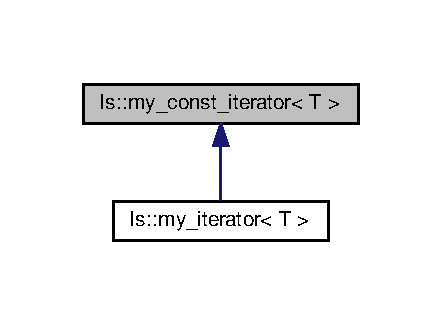
\includegraphics[width=212pt]{classls_1_1my__const__iterator__inherit__graph}
\end{center}
\end{figure}
\subsection*{Public Types}
\begin{DoxyCompactItemize}
\item 
\mbox{\Hypertarget{classls_1_1my__const__iterator_aa7aa8489a065e4ddda33727d33c84b7d}\label{classls_1_1my__const__iterator_aa7aa8489a065e4ddda33727d33c84b7d}} 
using \hyperlink{classls_1_1my__const__iterator_aa7aa8489a065e4ddda33727d33c84b7d}{value\+\_\+type} = T
\begin{DoxyCompactList}\small\item\em Alias to the constant data type. \end{DoxyCompactList}\item 
\mbox{\Hypertarget{classls_1_1my__const__iterator_aef920ed4e39e8680046437ad8d898d78}\label{classls_1_1my__const__iterator_aef920ed4e39e8680046437ad8d898d78}} 
using \hyperlink{classls_1_1my__const__iterator_aef920ed4e39e8680046437ad8d898d78}{pointer} = \hyperlink{classls_1_1my__const__iterator_aa7aa8489a065e4ddda33727d33c84b7d}{value\+\_\+type} $\ast$
\begin{DoxyCompactList}\small\item\em Pointer to the constant data type. \end{DoxyCompactList}\item 
\mbox{\Hypertarget{classls_1_1my__const__iterator_a47552bc9ef18669651047b1741c7ed42}\label{classls_1_1my__const__iterator_a47552bc9ef18669651047b1741c7ed42}} 
using \hyperlink{classls_1_1my__const__iterator_a47552bc9ef18669651047b1741c7ed42}{const\+\_\+reference} = \hyperlink{classls_1_1my__const__iterator_aa7aa8489a065e4ddda33727d33c84b7d}{value\+\_\+type} \&
\begin{DoxyCompactList}\small\item\em Referece to the constant data type. \end{DoxyCompactList}\item 
\mbox{\Hypertarget{classls_1_1my__const__iterator_a1808102357aa1f98d3da0ebccbb9e767}\label{classls_1_1my__const__iterator_a1808102357aa1f98d3da0ebccbb9e767}} 
using \hyperlink{classls_1_1my__const__iterator_a1808102357aa1f98d3da0ebccbb9e767}{difference\+\_\+type} = std\+::ptrdiff\+\_\+t
\begin{DoxyCompactList}\small\item\em Difference type to calculate the distance between two pointers. \end{DoxyCompactList}\end{DoxyCompactItemize}
\subsection*{Public Member Functions}
\begin{DoxyCompactItemize}
\item 
\mbox{\Hypertarget{classls_1_1my__const__iterator_a2465f5fcba843f6f65729e3d181b04f8}\label{classls_1_1my__const__iterator_a2465f5fcba843f6f65729e3d181b04f8}} 
\hyperlink{classls_1_1my__const__iterator_a47552bc9ef18669651047b1741c7ed42}{const\+\_\+reference} \& \hyperlink{classls_1_1my__const__iterator_a2465f5fcba843f6f65729e3d181b04f8}{operator$\ast$} () const
\begin{DoxyCompactList}\small\item\em Returns a const reference to the value stored in the iterator. \end{DoxyCompactList}\item 
\mbox{\Hypertarget{classls_1_1my__const__iterator_af058227856ecbcad2fe686a552ff2aec}\label{classls_1_1my__const__iterator_af058227856ecbcad2fe686a552ff2aec}} 
\hyperlink{classls_1_1my__const__iterator}{my\+\_\+const\+\_\+iterator} \& \hyperlink{classls_1_1my__const__iterator_af058227856ecbcad2fe686a552ff2aec}{operator++} ()
\begin{DoxyCompactList}\small\item\em Advances iterator to the next location within the list. Example\+: ++i;. \end{DoxyCompactList}\item 
\mbox{\Hypertarget{classls_1_1my__const__iterator_a13a2d927db55c7571ee2a6c835dc208b}\label{classls_1_1my__const__iterator_a13a2d927db55c7571ee2a6c835dc208b}} 
\hyperlink{classls_1_1my__const__iterator}{my\+\_\+const\+\_\+iterator} \hyperlink{classls_1_1my__const__iterator_a13a2d927db55c7571ee2a6c835dc208b}{operator++} (int)
\begin{DoxyCompactList}\small\item\em Advances iterator to the next location within the list. Example\+: i++;. \end{DoxyCompactList}\item 
\mbox{\Hypertarget{classls_1_1my__const__iterator_a44b566c18e94090b66101f604c17878e}\label{classls_1_1my__const__iterator_a44b566c18e94090b66101f604c17878e}} 
\hyperlink{classls_1_1my__const__iterator}{my\+\_\+const\+\_\+iterator} \& \hyperlink{classls_1_1my__const__iterator_a44b566c18e94090b66101f604c17878e}{operator-\/-\/} ()
\begin{DoxyCompactList}\small\item\em Advances iterator to the prev location within the list. Example\+: --i;. \end{DoxyCompactList}\item 
\mbox{\Hypertarget{classls_1_1my__const__iterator_a7064f57c440582a60281b7469b1bc5c9}\label{classls_1_1my__const__iterator_a7064f57c440582a60281b7469b1bc5c9}} 
\hyperlink{classls_1_1my__const__iterator}{my\+\_\+const\+\_\+iterator} \hyperlink{classls_1_1my__const__iterator_a7064f57c440582a60281b7469b1bc5c9}{operator-\/-\/} (int)
\begin{DoxyCompactList}\small\item\em Advances iterator to the prev location within the list. Example\+: i--;. \end{DoxyCompactList}\item 
\mbox{\Hypertarget{classls_1_1my__const__iterator_a8ff72b298122e39a7653e2619d23ea50}\label{classls_1_1my__const__iterator_a8ff72b298122e39a7653e2619d23ea50}} 
\hyperlink{classls_1_1my__const__iterator}{my\+\_\+const\+\_\+iterator} \hyperlink{classls_1_1my__const__iterator_a8ff72b298122e39a7653e2619d23ea50}{operator+} (int)
\begin{DoxyCompactList}\small\item\em Advances iterator to a specific position (walking throught the nodes). \end{DoxyCompactList}\item 
\mbox{\Hypertarget{classls_1_1my__const__iterator_a28c9d1af27e7e384338b1f9b2deeb7f1}\label{classls_1_1my__const__iterator_a28c9d1af27e7e384338b1f9b2deeb7f1}} 
bool \hyperlink{classls_1_1my__const__iterator_a28c9d1af27e7e384338b1f9b2deeb7f1}{operator==} (const \hyperlink{classls_1_1my__const__iterator}{my\+\_\+const\+\_\+iterator} \&rhs) const
\begin{DoxyCompactList}\small\item\em As in it1 == it2 \+: returns true if both iterators refer to the same location within the list, and false otherwise. \end{DoxyCompactList}\item 
\mbox{\Hypertarget{classls_1_1my__const__iterator_a73aba8c0843327b30e965555374a3c60}\label{classls_1_1my__const__iterator_a73aba8c0843327b30e965555374a3c60}} 
bool \hyperlink{classls_1_1my__const__iterator_a73aba8c0843327b30e965555374a3c60}{operator!=} (const \hyperlink{classls_1_1my__const__iterator}{my\+\_\+const\+\_\+iterator} \&rhs) const
\begin{DoxyCompactList}\small\item\em As in it1 != it2 \+: returns true if both iterators refer to a different location within the list, and false otherwise. \end{DoxyCompactList}\end{DoxyCompactItemize}
\subsection*{Protected Member Functions}
\begin{DoxyCompactItemize}
\item 
\mbox{\Hypertarget{classls_1_1my__const__iterator_a8ab448e804fac2d5117de8c8261a5873}\label{classls_1_1my__const__iterator_a8ab448e804fac2d5117de8c8261a5873}} 
\hyperlink{classls_1_1my__const__iterator_a8ab448e804fac2d5117de8c8261a5873}{my\+\_\+const\+\_\+iterator} (\hyperlink{structls_1_1Node}{Node}$<$ \hyperlink{classls_1_1my__const__iterator_aa7aa8489a065e4ddda33727d33c84b7d}{value\+\_\+type} $>$ $\ast$node=nullptr)
\begin{DoxyCompactList}\small\item\em Constructor. \end{DoxyCompactList}\end{DoxyCompactItemize}
\subsection*{Protected Attributes}
\begin{DoxyCompactItemize}
\item 
\mbox{\Hypertarget{classls_1_1my__const__iterator_a18548367e7f30dc4e358eff9172ba995}\label{classls_1_1my__const__iterator_a18548367e7f30dc4e358eff9172ba995}} 
\hyperlink{structls_1_1Node}{Node}$<$ T $>$ $\ast$ \hyperlink{classls_1_1my__const__iterator_a18548367e7f30dc4e358eff9172ba995}{current}
\begin{DoxyCompactList}\small\item\em Current node. \end{DoxyCompactList}\end{DoxyCompactItemize}
\subsection*{Friends}
\begin{DoxyCompactItemize}
\item 
\mbox{\Hypertarget{classls_1_1my__const__iterator_aa4cf6f043abfca0b41eb074c92dac6fa}\label{classls_1_1my__const__iterator_aa4cf6f043abfca0b41eb074c92dac6fa}} 
class {\bfseries list$<$ value\+\_\+type $>$}
\end{DoxyCompactItemize}


\subsection{Detailed Description}
\subsubsection*{template$<$typename T$>$\newline
class ls\+::my\+\_\+const\+\_\+iterator$<$ T $>$}

Constant iterator implementation. 

The documentation for this class was generated from the following file\+:\begin{DoxyCompactItemize}
\item 
include/list.\+h\end{DoxyCompactItemize}

\hypertarget{classls_1_1my__iterator}{}\section{ls\+:\+:my\+\_\+iterator$<$ T $>$ Class Template Reference}
\label{classls_1_1my__iterator}\index{ls\+::my\+\_\+iterator$<$ T $>$@{ls\+::my\+\_\+iterator$<$ T $>$}}


Implements the infrastructure to support the bidirectional pointer.  




{\ttfamily \#include $<$list.\+h$>$}



Inheritance diagram for ls\+:\+:my\+\_\+iterator$<$ T $>$\+:\nopagebreak
\begin{figure}[H]
\begin{center}
\leavevmode
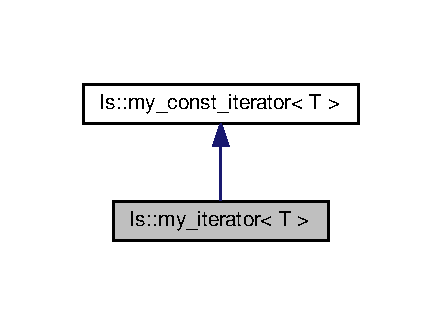
\includegraphics[width=212pt]{classls_1_1my__iterator__inherit__graph}
\end{center}
\end{figure}


Collaboration diagram for ls\+:\+:my\+\_\+iterator$<$ T $>$\+:\nopagebreak
\begin{figure}[H]
\begin{center}
\leavevmode
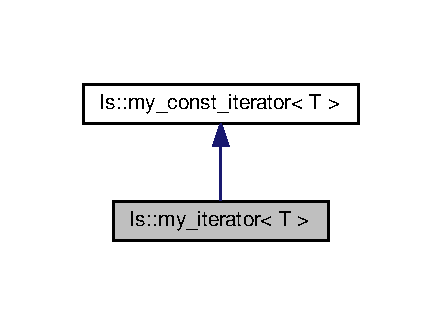
\includegraphics[width=212pt]{classls_1_1my__iterator__coll__graph}
\end{center}
\end{figure}
\subsection*{Public Types}
\begin{DoxyCompactItemize}
\item 
\mbox{\Hypertarget{classls_1_1my__iterator_aa67b52463c80c463dcb4919c3040903b}\label{classls_1_1my__iterator_aa67b52463c80c463dcb4919c3040903b}} 
using \hyperlink{classls_1_1my__iterator_aa67b52463c80c463dcb4919c3040903b}{value\+\_\+type} = T
\begin{DoxyCompactList}\small\item\em Alias to the data type. \end{DoxyCompactList}\item 
\mbox{\Hypertarget{classls_1_1my__iterator_a65792c5672e5b22715ec2b58c32e016a}\label{classls_1_1my__iterator_a65792c5672e5b22715ec2b58c32e016a}} 
using \hyperlink{classls_1_1my__iterator_a65792c5672e5b22715ec2b58c32e016a}{pointer} = \hyperlink{classls_1_1my__const__iterator_aa7aa8489a065e4ddda33727d33c84b7d}{value\+\_\+type} $\ast$
\begin{DoxyCompactList}\small\item\em Pointer to the data type. \end{DoxyCompactList}\item 
\mbox{\Hypertarget{classls_1_1my__iterator_ad3b5d3648d5b83344888204a9e6d7bfa}\label{classls_1_1my__iterator_ad3b5d3648d5b83344888204a9e6d7bfa}} 
using \hyperlink{classls_1_1my__iterator_ad3b5d3648d5b83344888204a9e6d7bfa}{reference} = \hyperlink{classls_1_1my__const__iterator_aa7aa8489a065e4ddda33727d33c84b7d}{value\+\_\+type} \&
\begin{DoxyCompactList}\small\item\em Referece to the data type. \end{DoxyCompactList}\item 
\mbox{\Hypertarget{classls_1_1my__iterator_a7a136fd439ffd4ed9d67a794d1001935}\label{classls_1_1my__iterator_a7a136fd439ffd4ed9d67a794d1001935}} 
using \hyperlink{classls_1_1my__iterator_a7a136fd439ffd4ed9d67a794d1001935}{const\+\_\+reference} = const \hyperlink{classls_1_1my__const__iterator_aa7aa8489a065e4ddda33727d33c84b7d}{value\+\_\+type} \&
\begin{DoxyCompactList}\small\item\em Reference to the constant data type. \end{DoxyCompactList}\item 
\mbox{\Hypertarget{classls_1_1my__iterator_a706553fcf9e3ea711d454eb7604aae1e}\label{classls_1_1my__iterator_a706553fcf9e3ea711d454eb7604aae1e}} 
using \hyperlink{classls_1_1my__iterator_a706553fcf9e3ea711d454eb7604aae1e}{difference\+\_\+type} = std\+::ptrdiff\+\_\+t
\begin{DoxyCompactList}\small\item\em Difference type to calculate the distance between two pointers. \end{DoxyCompactList}\end{DoxyCompactItemize}
\subsection*{Public Member Functions}
\begin{DoxyCompactItemize}
\item 
\mbox{\Hypertarget{classls_1_1my__iterator_ac18d9ac910a22e6b294edaecf86bfd19}\label{classls_1_1my__iterator_ac18d9ac910a22e6b294edaecf86bfd19}} 
\hyperlink{classls_1_1my__iterator_ac18d9ac910a22e6b294edaecf86bfd19}{my\+\_\+iterator} ()
\begin{DoxyCompactList}\small\item\em Constructor default. \end{DoxyCompactList}\item 
\mbox{\Hypertarget{classls_1_1my__iterator_ab8ae439a58cd299cbd364b3edf1dd855}\label{classls_1_1my__iterator_ab8ae439a58cd299cbd364b3edf1dd855}} 
\hyperlink{classls_1_1my__const__iterator_a47552bc9ef18669651047b1741c7ed42}{const\+\_\+reference} \& \hyperlink{classls_1_1my__iterator_ab8ae439a58cd299cbd364b3edf1dd855}{operator$\ast$} () const
\begin{DoxyCompactList}\small\item\em Return the constant data in that position. \end{DoxyCompactList}\item 
\mbox{\Hypertarget{classls_1_1my__iterator_a3eec7197d3d2b31cea843bc41b28451e}\label{classls_1_1my__iterator_a3eec7197d3d2b31cea843bc41b28451e}} 
\hyperlink{classls_1_1my__iterator_ad3b5d3648d5b83344888204a9e6d7bfa}{reference} \& \hyperlink{classls_1_1my__iterator_a3eec7197d3d2b31cea843bc41b28451e}{operator$\ast$} ()
\begin{DoxyCompactList}\small\item\em Return the data in that position. \end{DoxyCompactList}\item 
\mbox{\Hypertarget{classls_1_1my__iterator_aa958375bc05acb1767e82e69373c9a25}\label{classls_1_1my__iterator_aa958375bc05acb1767e82e69373c9a25}} 
\hyperlink{classls_1_1my__iterator}{my\+\_\+iterator} \& \hyperlink{classls_1_1my__iterator_aa958375bc05acb1767e82e69373c9a25}{operator++} ()
\begin{DoxyCompactList}\small\item\em Advances iterator to the next location within the list. Example\+: ++i;. \end{DoxyCompactList}\item 
\mbox{\Hypertarget{classls_1_1my__iterator_a87cd11c26f7cff8fb68631d100354143}\label{classls_1_1my__iterator_a87cd11c26f7cff8fb68631d100354143}} 
\hyperlink{classls_1_1my__iterator}{my\+\_\+iterator} \hyperlink{classls_1_1my__iterator_a87cd11c26f7cff8fb68631d100354143}{operator++} (int)
\begin{DoxyCompactList}\small\item\em Advances iterator to the next location within the list. Example\+: i++;. \end{DoxyCompactList}\item 
\mbox{\Hypertarget{classls_1_1my__iterator_a27cc5599241072286f87eb3a05275dce}\label{classls_1_1my__iterator_a27cc5599241072286f87eb3a05275dce}} 
\hyperlink{classls_1_1my__iterator}{my\+\_\+iterator} \& \hyperlink{classls_1_1my__iterator_a27cc5599241072286f87eb3a05275dce}{operator-\/-\/} ()
\begin{DoxyCompactList}\small\item\em Advances iterator to the prev location within the list. Example\+: --i;. \end{DoxyCompactList}\item 
\mbox{\Hypertarget{classls_1_1my__iterator_a4e31b9ed0b69c94db7027415c1ad5192}\label{classls_1_1my__iterator_a4e31b9ed0b69c94db7027415c1ad5192}} 
\hyperlink{classls_1_1my__iterator}{my\+\_\+iterator} \hyperlink{classls_1_1my__iterator_a4e31b9ed0b69c94db7027415c1ad5192}{operator-\/-\/} (int)
\begin{DoxyCompactList}\small\item\em Advances iterator to the prev location within the list. Example\+: i--;. \end{DoxyCompactList}\item 
\mbox{\Hypertarget{classls_1_1my__iterator_a77ccb3303f10b6930457fd090c4f2187}\label{classls_1_1my__iterator_a77ccb3303f10b6930457fd090c4f2187}} 
\hyperlink{classls_1_1my__iterator}{my\+\_\+iterator} \hyperlink{classls_1_1my__iterator_a77ccb3303f10b6930457fd090c4f2187}{operator+} (int)
\begin{DoxyCompactList}\small\item\em Advances iterator to a specific position (walking throught the nodes). \end{DoxyCompactList}\item 
\mbox{\Hypertarget{classls_1_1my__iterator_af87392d8c1ad98e669827f622771053a}\label{classls_1_1my__iterator_af87392d8c1ad98e669827f622771053a}} 
bool \hyperlink{classls_1_1my__iterator_af87392d8c1ad98e669827f622771053a}{operator$<$} (\hyperlink{classls_1_1my__iterator}{my\+\_\+iterator} \&) const
\begin{DoxyCompactList}\small\item\em Verifies if a element is less then another. \end{DoxyCompactList}\item 
\mbox{\Hypertarget{classls_1_1my__iterator_a7582cc03e5885a77599f509dd06bb0cf}\label{classls_1_1my__iterator_a7582cc03e5885a77599f509dd06bb0cf}} 
bool \hyperlink{classls_1_1my__iterator_a7582cc03e5885a77599f509dd06bb0cf}{operator==} (\hyperlink{classls_1_1my__iterator}{my\+\_\+iterator} \&rhs) const
\begin{DoxyCompactList}\small\item\em As in it1 == it2 \+: returns true if both iterators refer to the same location within the list, and false otherwise. \end{DoxyCompactList}\item 
\mbox{\Hypertarget{classls_1_1my__iterator_a57a517f86159fc752b74b06a73fdfa68}\label{classls_1_1my__iterator_a57a517f86159fc752b74b06a73fdfa68}} 
bool \hyperlink{classls_1_1my__iterator_a57a517f86159fc752b74b06a73fdfa68}{operator!=} (\hyperlink{classls_1_1my__iterator}{my\+\_\+iterator} \&rhs) const
\begin{DoxyCompactList}\small\item\em As in it1 != it2 \+: returns true if both iterators refer to a different location within the list, and false otherwise. \end{DoxyCompactList}\end{DoxyCompactItemize}
\subsection*{Friends}
\begin{DoxyCompactItemize}
\item 
\mbox{\Hypertarget{classls_1_1my__iterator_aa4cf6f043abfca0b41eb074c92dac6fa}\label{classls_1_1my__iterator_aa4cf6f043abfca0b41eb074c92dac6fa}} 
class {\bfseries list$<$ value\+\_\+type $>$}
\end{DoxyCompactItemize}
\subsection*{Additional Inherited Members}


\subsection{Detailed Description}
\subsubsection*{template$<$typename T$>$\newline
class ls\+::my\+\_\+iterator$<$ T $>$}

Implements the infrastructure to support the bidirectional pointer. 

The documentation for this class was generated from the following file\+:\begin{DoxyCompactItemize}
\item 
include/list.\+h\end{DoxyCompactItemize}

\hypertarget{structls_1_1Node}{}\section{ls\+:\+:Node$<$ T $>$ Struct Template Reference}
\label{structls_1_1Node}\index{ls\+::\+Node$<$ T $>$@{ls\+::\+Node$<$ T $>$}}


Structure to each element in the list.  




{\ttfamily \#include $<$list.\+h$>$}

\subsection*{Public Member Functions}
\begin{DoxyCompactItemize}
\item 
\mbox{\Hypertarget{structls_1_1Node_a9d72765459432e7e6ed9d4774fde5bc9}\label{structls_1_1Node_a9d72765459432e7e6ed9d4774fde5bc9}} 
\hyperlink{structls_1_1Node_a9d72765459432e7e6ed9d4774fde5bc9}{Node} (const T \&d=T(), \hyperlink{structls_1_1Node}{Node} $\ast$p=nullptr, \hyperlink{structls_1_1Node}{Node} $\ast$n=nullptr)
\begin{DoxyCompactList}\small\item\em \hyperlink{structls_1_1Node}{Node}\textquotesingle{}s constructor default. \end{DoxyCompactList}\end{DoxyCompactItemize}
\subsection*{Public Attributes}
\begin{DoxyCompactItemize}
\item 
\mbox{\Hypertarget{structls_1_1Node_ab1c22709e50c994125d21f1998b3b3b7}\label{structls_1_1Node_ab1c22709e50c994125d21f1998b3b3b7}} 
T \hyperlink{structls_1_1Node_ab1c22709e50c994125d21f1998b3b3b7}{data}
\begin{DoxyCompactList}\small\item\em The informations to be stored. \end{DoxyCompactList}\item 
\mbox{\Hypertarget{structls_1_1Node_a36cbf598150b7e4c7708933f78252b65}\label{structls_1_1Node_a36cbf598150b7e4c7708933f78252b65}} 
\hyperlink{structls_1_1Node}{Node}$<$ T $>$ $\ast$ \hyperlink{structls_1_1Node_a36cbf598150b7e4c7708933f78252b65}{prev}
\begin{DoxyCompactList}\small\item\em Previous node. \end{DoxyCompactList}\item 
\mbox{\Hypertarget{structls_1_1Node_a969a6cf64494340df3bd7136b4e7daca}\label{structls_1_1Node_a969a6cf64494340df3bd7136b4e7daca}} 
\hyperlink{structls_1_1Node}{Node}$<$ T $>$ $\ast$ \hyperlink{structls_1_1Node_a969a6cf64494340df3bd7136b4e7daca}{next}
\begin{DoxyCompactList}\small\item\em Next node. \end{DoxyCompactList}\end{DoxyCompactItemize}


\subsection{Detailed Description}
\subsubsection*{template$<$typename T$>$\newline
struct ls\+::\+Node$<$ T $>$}

Structure to each element in the list. 

The documentation for this struct was generated from the following file\+:\begin{DoxyCompactItemize}
\item 
include/list.\+h\end{DoxyCompactItemize}

%--- End generated contents ---

% Index
\backmatter
\newpage
\phantomsection
\clearemptydoublepage
\addcontentsline{toc}{chapter}{Índice}
\printindex

\end{document}
